\documentclass[reprint,norsk,notitlepage,floatfix]{revtex4-2}
\usepackage{amsmath}
\usepackage[mathletters]{ucs}
\usepackage[utf8x]{inputenc}
\usepackage[norsk]{babel}
\usepackage{esint}
\usepackage{physics,amssymb}
\usepackage{graphicx}
\usepackage{xcolor}
\usepackage[colorlinks=true]{hyperref}
\usepackage{cleveref}
\usepackage{listings}
\usepackage{enumitem}
\usepackage{subfigure}
\usepackage{float}
\usepackage{array, booktabs}
\newcolumntype{C}[1]{>{\centering\let\newline\\\arraybackslash\hspace{0pt}}m{#1}}
\newcommand\numberthis{\addtocounter{equation}{1}\tag{\theequation}}

\usepackage{sectsty}

\newcommand{\TODO}[1]{}
% \usepackage[style=science, backend=biber]{biblatex}
% \addbibresource{References_Part_4.bib} TODO: Slett før innlevering
\hypersetup{
    colorlinks,
    linkcolor={red!50!black},
    citecolor={blue!50!black},
    urlcolor={blue!80!black}}

\lstset{inputpath=,
    backgroundcolor=\color{white!88!black},
    basicstyle={\ttfamily\scriptsize},
    commentstyle=\color{magenta},
    language=Python,
    morekeywords={True,False},
    tabsize=4,
    stringstyle=\color{green!55!black},
    frame=single,
    keywordstyle=\color{blue},
    showstringspaces=false,
    columns=fullflexible,
    keepspaces=true}

\begin{document}

\title{Lab Rapport: Bølgeoptikk}
\author{Kandidat: 127}
\date{\today}
\affiliation{}



\begin{abstract}
    Hensikten med forsøkene gjennomført i denne rapporten er å studere interferens, diffraksjon og brytning av lys. Dette ble gjort ved å sende lys gjennom enkelt og dobbelt-spalter samt sirkulær apertur, og sammenligning av teoretiske beregninger med eksperimentelle resultater. Videre så vi på hvordan lys av forskjellige bølgelengder brytes ved møte ved et gitter, og hvordan vi kan regne oss tilbake til bølgelengden ved bruk av observert vinkel. Til slutt studerte vi Zeeman-effekten hvor et magnetfelt fører til oppdeling av degenererte energinivåer, som skapte et nytt interferensmønster vi kunne bruke for å finne differansen i frekvens. Vi klarte i varierende grad å beregne oss tilbake til teoretiske verdier. Her var beregningen av Bohr-magnetonet $μ_B$ veldig nære med bare $0.55\%$ avvik for den ene beregningen. Beregningene for bølgelengdene til emmisjonspekterert til helium og hydrogen var også veldig nøyaktig og innenfor våre usikkerheter. De største feilene oppstod når vi undersøkte avstander mellom sentrum og lysmaksima for forskjellige typer spalter. Her burde vi ha anslått en større usikkerhet i våre målinger. 
    % TODO: Legg til mer resultater
\end{abstract}
\maketitle

\section{Introduksjon} \label{sec: introduksjon}
  Et av de mest grunnleggende egenskapene til lys, er dets kombinasjon av bølge- og partikkelegenskaper. Dette fører til mange effekter som interferens, diffraksjon, spektrallinjer og varierende avbøyning ved møte med gitter, avhengig av bølgelengde. Dette påvirker flere fenomener på stor og liten skala i universet. Derfor er det å få god forståelse for disse effektene helt vesentlig for forståelse og modellering av universet. 
  
  Fokuset for forsøkene vi skal gjennomføre er forskjell i intensitet i interferensmønster som kan beskrives ved illumninansfunksjoner, og lys emittert basert på energiforskjeller basert på Bohr's atommodell. Vi skal bruke spalter med kjente verdier til å lage forskjellige diffraksjonsmønster, og regne oss tilbake til de kjente verdiene. Dette gjøres for å bekrefte de teoretiske modellene vi bruker for å beskrive disse fenomenene. Vi starter ved å lage interferensmønster med monokromatisk lys med kjent bølgelengde, og kjente spalteavstander. Her håper vi ved bruk av teoretiske modeller å finne tilbake til spaltebreddene. 
  
  Videre bruker vi eksitert helium og hydrogen gass som emitterer kjente bølgelengder. Disse avbøyes av et gitter med, hvor avbøyningsvinkel er avhengig av bølgelengde. Vi skal da notere oss vinkelen og se hvor nært våre beregninger kommer de kjente bølgelengde
  
  Til slutt skal vi beregne den kjente Bohr-magnetonet $μ_B$ ved differanse i frekvens skapt av den normale Zeeman-effekten hvor degenererte energinivåer splittes opp i et magnetfelt. 
  

\section{Teori} \label{sec: teori}
  \subsection{Interferens og diffraksjon ved passering av spalter}
    Lys oppfører seg både som partikkel og bølge avhengig av hvordan det måles. Når lys passerer én eller flere spalter vil, hvis spalten er liten nok, det oppstå et interferens mønster. Dette kan forklares ved Huygens prinsipp
    hvor et hvert punkt på en bølgefront kan sees som en kilde til en elementærbølge. Disse bølgene vil interferere med hverandre, og dermed skape et interferensmønster. Dette mønsteret kan observeres på en skjerm bak spalten som områder av varierende intensitet. Intensiteten er beskrevet av \textit{Illumninansfunksjonen} \cref{eq: illuminansfunksjon}. 
    \begin{equation}\label{eq: illuminansfunksjon}
      E_{N}(x) = E_1(x) F_N(x)
    \end{equation} 
    hvor $N$ er antall spalter, $x$ er horisontal avstanden fra sentrum. Vi bruker tre forskjellige typer spalter i våre forsøk. 
    
    \subsubsection*{Én spalte}
      Når vi bare har én spalte er $N = 1$, er illuminansen beskrevet ved \cref{eq: E_1} 
      \begin{equation}\label{eq: E_1}
        E_1(x) \propto \frac{\sin^2 (acx)}{(acx)^2}
      \end{equation}
      hvor $c = π / λR$. I områdene med totalt destruktiv interferens vil det være mørkt. Avstanden $x$ mellom disse områdene fra sentrum er gitt ved 
      \begin{equation}\label{eq: lysminima}
        x = \frac{nλR}{a}
      \end{equation}
      hvor $n ∈ ℕ \setminus \left\{0\right\}$, $λ$ er bølgelengden til lyset, $R$ er avstanden mellom spalten og skjermen, og $a$ er bredden til spalten. Dette er derivert fra nullpunktene fra  \cref{eq: E_1}. 
      
    \subsubsection*{N spalter}
    Hvis lyset passerer gjennom $N$ spalter med en avstand $A$ mellom hver spalte, oppfører hver spalte seg som en kilde til bølger, som igjen vil interfere med hverandre. Dette kombineres til en superposisjon av bølger, hvor illuminansen er beskrevet av \cref{eq: E_N}. 
    \begin{equation}\label{eq: E_N}
      E_1(x) F_N(x) \propto \left(\frac{\sin (acx)}{acx}\right)^2 \left(\frac{\sin (NAcx)}{\sin Acx}\right)^2
    \end{equation}
    Videre får vi dermed lokale hovedmaksima hvor illuminansen er høyest, for $x$ gitt ved \cref{eq: lysmaksima}, og lysminima for $x$ gitt ved \cref{eq: N lysminima}.
     
    \begin{equation}\label{eq: lysmaksima}
      x = \frac{mλR}{A}, \quad m ∈ ℤ
    \end{equation}
    
    \begin{equation}\label{eq: N lysminima}
      x = \frac{λR}{A} \left(\frac{1}{N}, \frac{2}{N},\ldots , \frac{N-1}{N}, \frac{N+1}{N},\ldots  \right)
    \end{equation}
    \subsubsection*{Sirkulær apertur}
      Når lys passerer gjennom et stort og sirkulært hull, vil det oppstå sirkulære interferensmønster. I et plan ved stor avstand $R$ fra hullet er illuminansen $H(ω)$ gitt ved \cref{eq: H}
      \begin{equation}\label{eq: H}
        H(ω) \propto \left(\frac{2J_1(ω)}{ω}\right)^2 , \quad ω = \frac{πar}{λR}
      \end{equation}
      hvor $J_1$ er Besselfunksjonen av første orden og $r$ er radiell avstand fra mønsterets sentrum. $H(ω)$ har nullpunkter for $ω_0 ∈ \left\{3.832, 7.016, 13.324\right\}$ 
      
      \begin{figure}[h!]
        \centering
        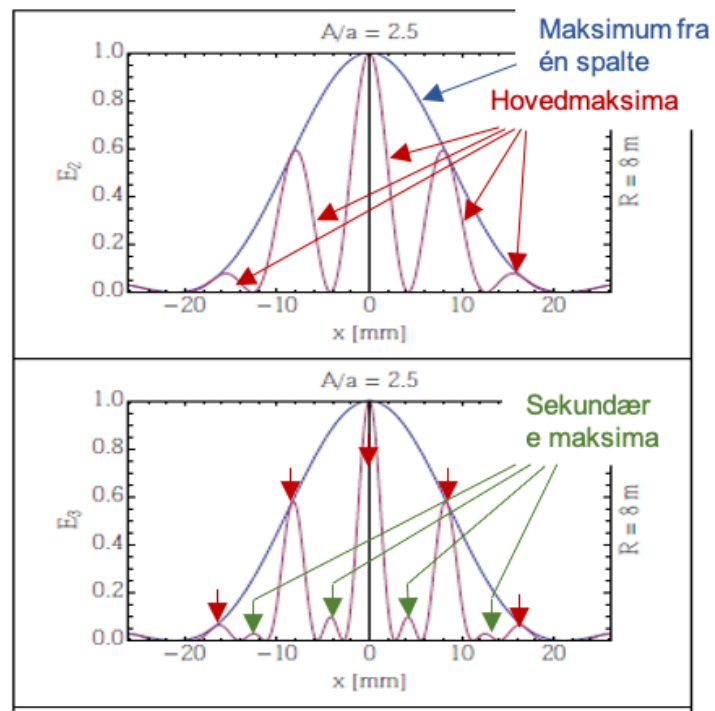
\includegraphics[width = .45\textwidth]{Maksima.png}
        \caption{Illustrasjon av forskjellige typer maksima for enkelt og flere spalter hentet fra \ref{source: lab}}
        \label{fig: maksima}
      \end{figure}
    
  \subsection{Gitterspektroskopi}
    Lys med forskjellige bølgelengder kan skilles ved å la de passere et lite gitter med avstand $d$. Det er fordi de blir avbøyd forskjellig, avhengig av bølgelengden som illustrert i \cref{fig: gitter}. En kan observere at laver bølgelengder har lavere avbøyninngsvinkler, enn høyere bølgelengder.  
    
    \begin{figure}[h!]
      \centering
      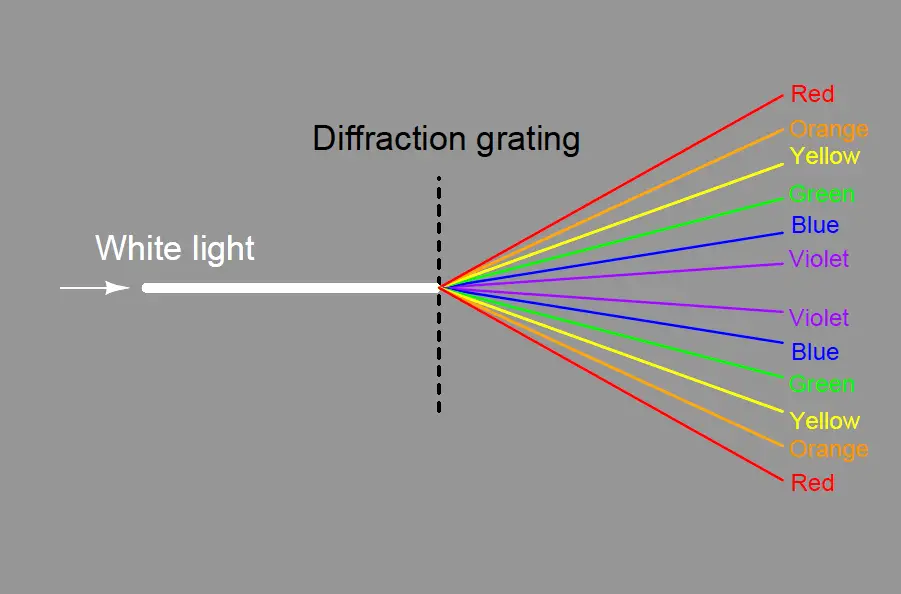
\includegraphics[width = .45\textwidth]{diffraction-grating.png}
      \caption{Illustrasjon av lys som passerer gjennom et gitter, hentet fra \ref{source: diffraction}}
      \label{fig: gitter}
    \end{figure}
    
    Ettersom det benyttes veldig mange spalter, vil en nesten bare observere hovedmaksima for hver bølgelengde gitt ved \cref{eq: illuminansfunksjon}, ettersom illuminansen til de sekundære maksimaene er mye mindre. Hvis en anntar at $\left|x\right| ≪ R$ kan vi skrive om $\displaystyle \frac{x}{R} ≈ \frac{x}{\sqrt{R^2 + x^2}} = \sin θ$, hvor $θ$ er avbøyningsvinkelen. Da kan vi skrive om \cref{eq: illuminansfunksjon} til \cref{eq: illuminansfunksjon2}.
    
    \begin{equation}\label{eq: illuminansfunksjon2}
      d\sin θ = mλ
    \end{equation}
    der $d$ er gitterkonstanten (gitter per lengdeenhet), og $m$ er spekterets orden (antall kopier av samme bølgelengde på hver side av innkommende akse). For å utforske dette fenomenet, brukes et \textit{gitterspektrometer}
    
    \subsubsection*{Gitterspektrometer}
      Et gitterspektrometer av flere deler som lar oss observere avbøyningsvinkelen til forskjellige bølgelengder. Når en gass eksisteres vil dets elektroner hoppe opp i energinivå, og emittere lys når det faller ned igjen. For noen atomer er dette i det synlige spekteret og en vil se gassen gløde. En kollimator har i oppgave å samle dette lyset, ved bruk av en konveks linse, til en bunt som sendes vinkelrett på gitteret. Spektrallinjen som inneholder gassen er plassert i linsen sitt brennplan. Gitteret splitter lyset opp med forskjellig avbøyningsvinkel avhengig av bølgelengde. Da brukes et teleskop på andre siden som kan roteres for å observere de forskjellige bølgelengdene, én etter én. Ettersom lyset kommer inn parallelt med optisk akse er teleskopet innstilt med et fokus "uendelig" langt unna. På mekanismen som lar oss rotere teleskopet er det en gradskive. Ved bruk av den samt et tynt trådkors på linsen kan en notere observert vinkel for hver bølgelengde. Får å redusere usikkerheten i målingene bør en notere vinkelen for hver bølgelengde på både høyre og venstre side av innkommende akse. Da kan en ta gjennomsnittet av de to målingene for å få en mer nøyaktig verdi som vist i \cref{eq: avg_angle}.
      
      \begin{equation}\label{eq: avg_angle}
        θ = \frac{α_h - α_v}{2}
      \end{equation}
      
      Vi får en usikkerhet i bølgelengden som vist i \cref{eq: usikkerhet_lambda}
      
      \begin{equation}\label{eq: usikkerhet_lambda}
        \frac{λ}{Δλ} = \sqrt{\left(\frac{Δd}{d}\right)^2 + \left(\frac{Δθ}{\tan θ}\right)^2}
      \end{equation}
      Usikkerheten i gitterkonstanten $d$ er som regel neglisjerbar. Da kan en sette $Δd = 0$ og vi får $Δθ$ uttrykket ved \cref{eq: usikkerhet_theta}
      
      \begin{equation}\label{eq: usikkerhet_theta}
        Δθ = \frac{1}{2} \sqrt{(Δα_h)^2 + (Δα_v)^2}
      \end{equation}
      
      Vi får en gitteroppløsning som beksrevet i \cref{eq: gitter opplosning}
      
      \begin{equation}\label{eq: gitter opplosning}
        \frac{λ}{Δλ} = mN ⇒ Δλ = \frac{λ}{mN}
      \end{equation}
      
    \subsubsection*{Emisjonspekter}
      Når elektroner for så å falle fra et skall med høyere energi, til et med lavere energi, vil det også emmitere et foton med energi tilsvarende energitapet fra hoppet. For hydrogen og helium er de forskjellige kombinasjonene av hopp fra et skall til et annet godt kjent. Dette gir oss et klart emisjonsspektrum som er distinkt for hver gass. Dette er illustrert i \cref{fig: emisjonsspekter}. 
      
      \begin{figure}[h!]
        \centering
        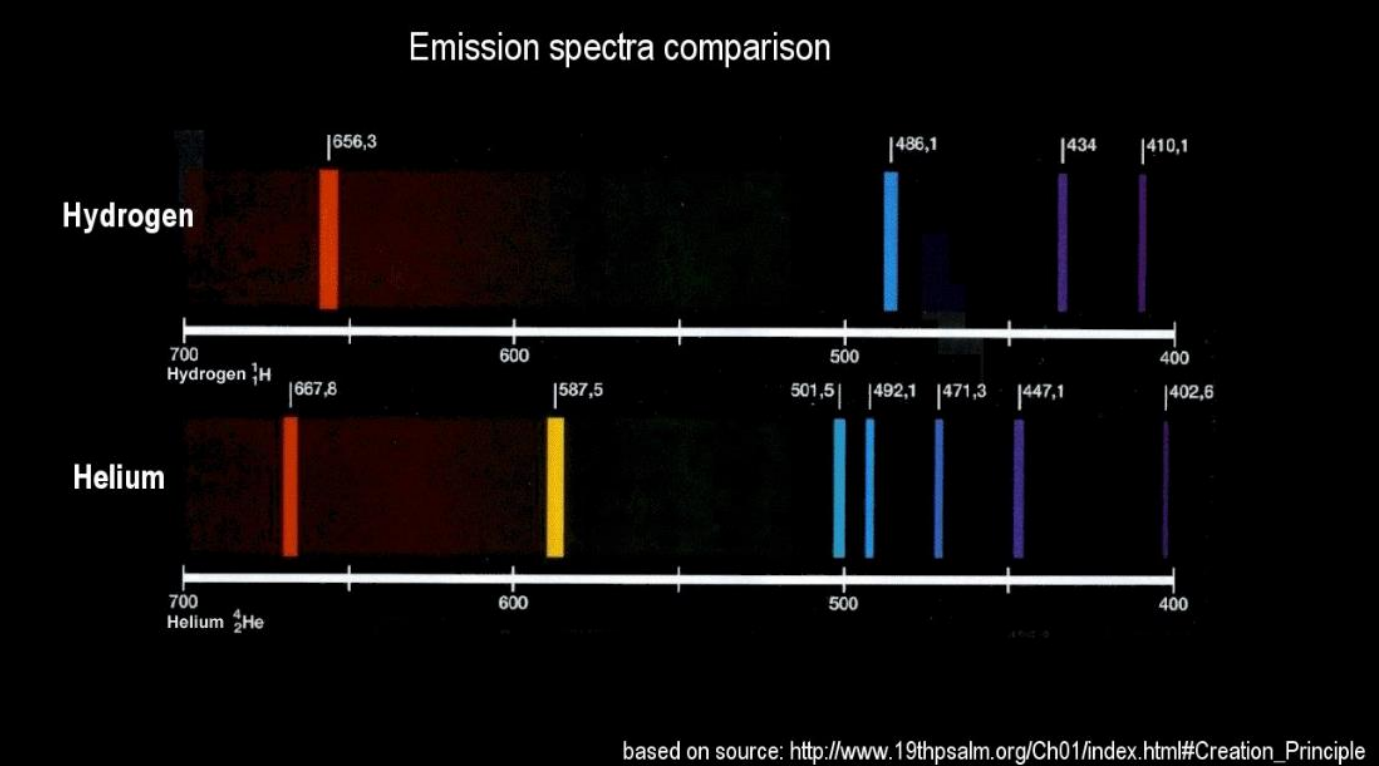
\includegraphics[width = .45\textwidth]{emisjon.png}
        \caption{Emisjonspekter for hydrogen og helium, hentet fra lab instruks \ref{source: lab}}
        \label{fig: emisjonsspekter}
      \end{figure}
      
      
  \subsection{Zeeman effekten}
    Når et elektron eksisteres for så falle fra et høyere energinivå til et lavere, emitterer det et foton med energi (og tilhørende bølgelengde), proporsjonalt med differansen i potensiell energi, mellom de to elektronskallene. Dette fører til diskrete spektrallinjer. Den potensielle energien er da bare bestemt av det prinsipielle kvantetallet $n ∈ N \setminus \left\{0\right\}$, som beskriver hvilket hoved-skall elektronet befinner seg i, og det asimutale kvantetallet $l ∈ [0, n-1]∩ℤ$ som bestemmer hvilket underskall elektronet befinner seg i. Plassert i et magnetfelt, vil den potensielle energien $V_{nl}$ til elektronet også være avhengig av spinn-kvantetallet $m_s$, som for elektroner er $\pm 1 / 2$, og det magnetiske kvantetallet $m_l ∈ [-l, l]∩ℤ$.
    
    For et elektron med masse $m_e$ og ladning $e$ plassert i et homogent magnetfelt med styrke $B$, vil den potensielle energien få et lite bidrag $V_s$ fra spinnet gitt ved \cref{eq: V_ms}
    
    \begin{equation}\label{eq: V_ms}
      V_{m_s} = μB = \frac{eBℏ}{2m_e}g m_s = ± \frac{eBℏ}{2m_e}
    \end{equation}
    der $ℏ$ er den reduserte Plack konstanten og $g$ er Landé g-faktoren. For elektroner er $g = 2$. Det samme elektronet vil også få et bidrag $V_{m_l}$ gitt ved \cref{eq: V_ml}
    
    \begin{equation}\label{eq: V_ml}
      V_{m_l} = m_l μ_B B
    \end{equation}
    der $μ_B$ er Bohr-magneton. 
    
    For kadmium vil vi bare observere den \textit{normale Zeeman effekten}, hvor en bare får et bidrag $V_{m_l}$. Vi skal bare se på fotonene emittert fra elektroner som hopper fra $l=2$ til $l=1$. Hvis atomet ikke er i et magnetfelt, ville de bare kunne emittert fotoner med samme energi, ettersom $m_l$ ikke påvirker energien. Ettersom atomene er i et magnetfelt får vi 9 mulige hopp i energi, ettersom vi har 5 mulige $m_l$ når $l=2$ og 3 mulige $m_l$ når $l=1$.
  
    Ettersom de emitterte lysstrålene har litt forskjellig energi $ΔE$ vil de ha litt forskjellig frekvens gitt ved \cref{eq: delta_E}
    
    \begin{equation}\label{eq: delta_E}
      ΔE = h ν
    \end{equation}
    der $h$ er Plack konstanten og $ν$ er frekvensen til fotonet. Dette gir en frekvensforskjell $Δν$ gitt ved \cref{eq: delta_nu}. 

    \begin{equation}\label{eq: delta_nu}
      Δν = \frac{2μ_B B}{h}
    \end{equation}
    
    Denne endringen er veldig liten så for å skille de forskjellige frekvensene bruker vi et \textit{Fabry-Pérot interferometer}. 
    
    \subsubsection*{Fabry-Pérot Interferometer}
      FP-interferometer bruker interferens mellom parallelle, semitransparente tynne plater med en avstand $t ≈ 2.9 ± 0.1$ mm. Disse platene gjør at noe av lyset reflekteres flere ganger, mens noe av lyset går rett igjennom. Dette gjør at lyset interferer med seg selv og bare noen bølgelengder $λ$ får passere gitt ved \cref{eq: FP interference}.
      
      \begin{equation}\label{eq: FP interference}
        nλ = 2t \cos θ ≈ 2t, \quad n ∈ ℕ
      \end{equation} 
      
      Videre passerer lyset gjennom en linse med brennvidde $f = 100$ mm, og inn i en kameralinse. På linsen vil vi observere et sirkulært diffraksjonsmønster med radius $r = f \tanθ$. Lyset er planpolarisert og lyset til fotonene fra elektronene med $m_l = 0$ står normalt på fotonene fra elektronene med $m_l ≠ 0$. Disse kan vi filtrere ut med et polarisasjonsfilter. Da observerer vi bare linjene med frekvens $ν_a$ og $ν_b$ fra $m_l ≠  0$. Dette kan vi igjen bruke for å finne frekvensforskjellen $Δν$ gitt ved \cref{eq: delta nu}. 
      
      \begin{equation}\label{eq: delta nu}
        Δν = ν_a - ν_b = \frac{2μ_B B}{h} = \frac{c}{2t} \underbrace{\frac{d_2^2 - d_1^2}{d_3^2 - d_1^2}}_{δ}
      \end{equation}
      hvor $d_n$ er diameteren til den $n$-te ringen og $δ$ er nøkkelparameteren. 
      
      Ved en fast usikkerhet $Δd^{±}$ som er konstant for alle diametere får vi en usikkerhet $Δd$ gitt ved \cref{eq: delta d}.
      
      \begin{equation}\label{eq: delta d}
        \Delta d = \sqrt{\left(\frac{\Delta d^\pm}{2}\right)^2 + \left(\frac{\Delta d^\pm}{2}\right)^2} = \frac{\Delta d^{\pm}}{2}
      \end{equation}
      
      Når vi kombinerer dette for flere diametere får vi en total usikkerhet i nøkkelparameteren $δ$ gitt ved \cref{eq: delta d total}.
      
      \begin{equation}\label{eq: delta d total}
        Δδ = Δd^{±}\sqrt{\frac{d_2^2 + d_1^2}{\Delta d_{2,1}^2} + \frac{d_3^2 + d_1^2}{\Delta d_{3,1}^2}} 
      \end{equation}
    
      Vi finner beregner Bohr-magnetonet ved \cref{eq: bohr magneton}.
      
      \begin{equation}\label{eq: bohr magneton}
        μ_B = \frac{hΔν}{2B}
      \end{equation}
      
      
      Magnetfeltet $B$ har forskjellig styrke basert på plassering mellom elektromagnetene. Dette har blitt beregnet og notert i \ref{fig: feltstyrke}
      
      \begin{figure}[h!]
        \centering
        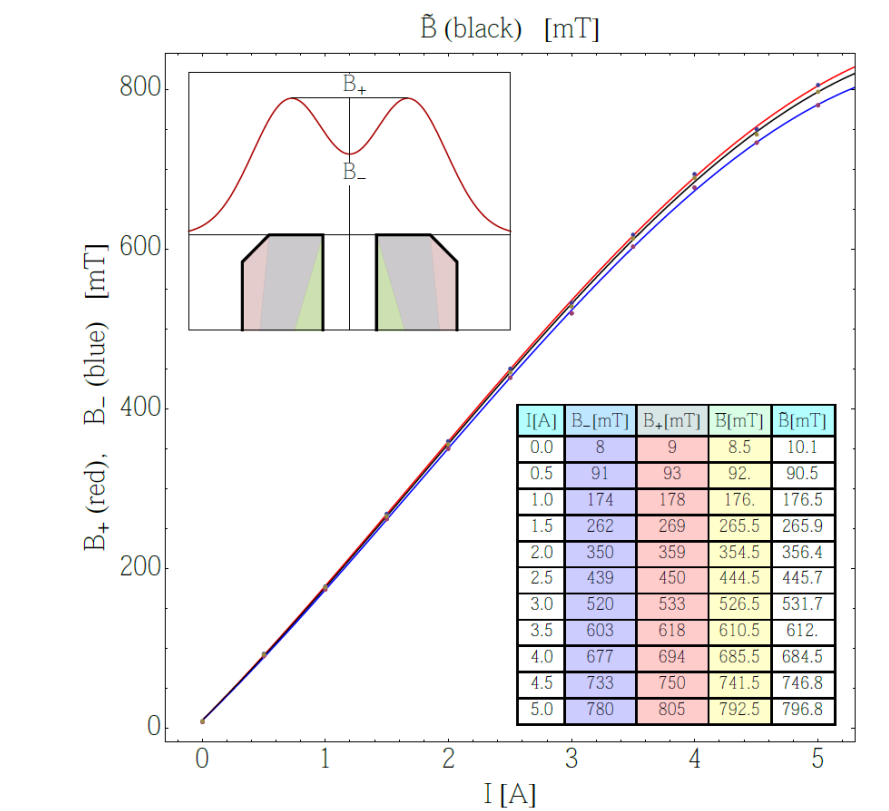
\includegraphics[width = .45\textwidth]{magnetstyrke.png}
        \caption{Feltstyrke som funksjon av strøm og plassering mellom elektromagnetene. Hentet fra lab instruks \ref{source: lab}}
        \label{fig: feltstyrke}
      \end{figure}
  
    \subsection{Beregning av usikkerheter}
      \begin{figure}[h!]
        \centering
        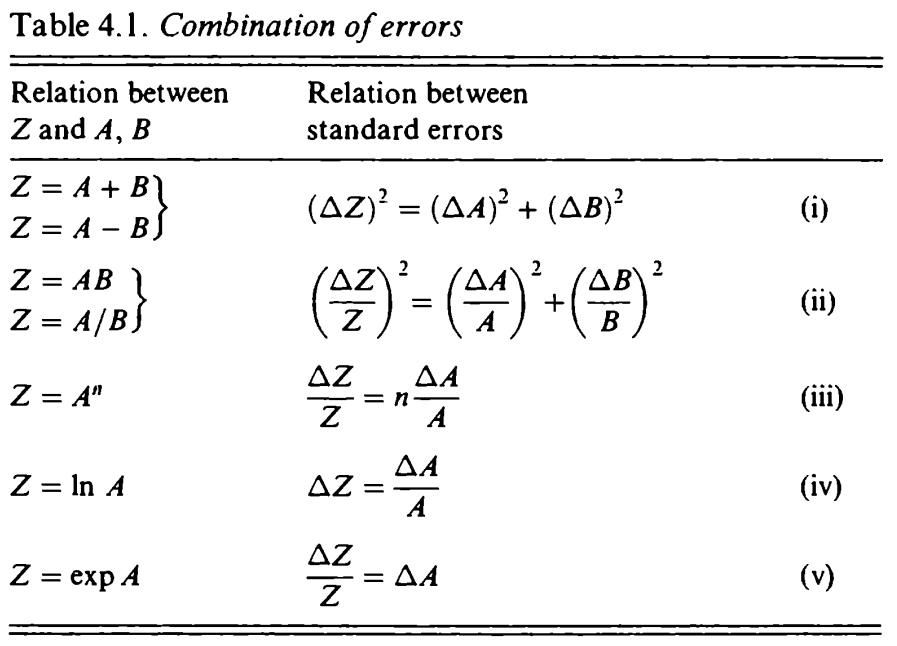
\includegraphics[width = .45\textwidth]{Usikkerheter.png}
        \caption{Formler for beregning av usikkerheter hentet fra side 29 i Squires \ref{source: squire}}
        \label{fig: usikkerheter}
      \end{figure}
    
    

  % TODO: Skriv om hvordan plassering i magnetfeltet påvirker zeeman effekten, og gå over kalibreringen som vist på side 12


\section{Eksperimentelt} \label{sec: eksperimentelt}
  \subsection{Diffraksjonsmønster ved HeNe Laser}
    \begin{figure}[h!]
      \centering
      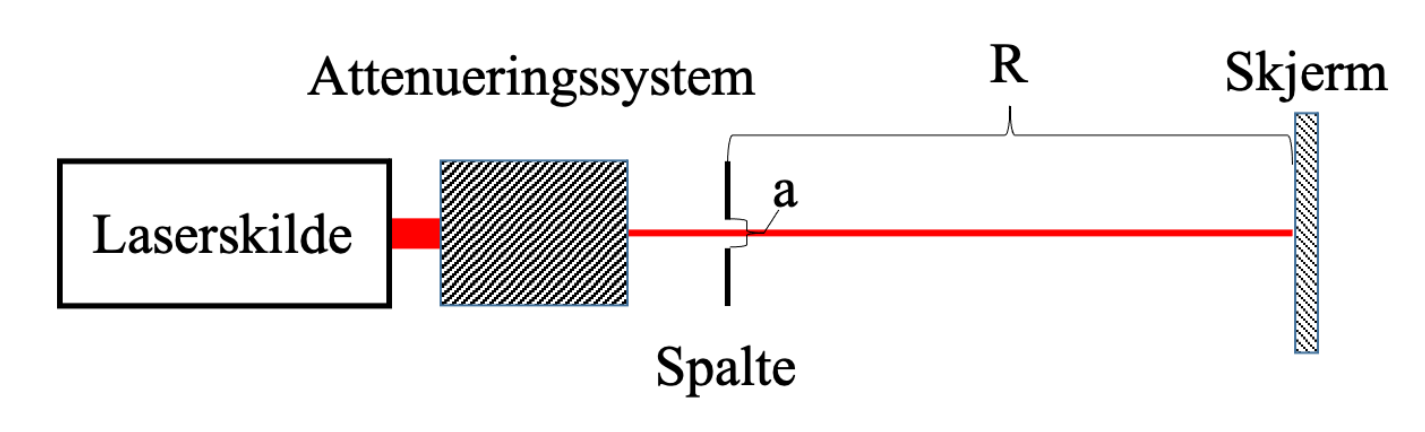
\includegraphics[width = .45\textwidth]{Oppsett_A.png}
      \caption{Illustrasjon av oppsett for observasjon av diffraksjonsmønster ved HeNe laser hentet fra \ref{source: lab}.}
      \label{fig: oppsett_A}
    \end{figure}

    Vi begynte med å sette opp laseren, med bølgelengden $λ = 632.8$ nm, en avstand $R = 0.576$ m unna et hvitt ark. Avstanden ble målt ved Bosch PLR 30 digital lasermåler som har en usikkerhet på $2$ mm.  
    Laseren gikk deretter gjennom enkelt, dobbelt og sirkulære spalter. Spaltene brukt hadde kjente størrelser for spaltebredde $a$ og avstand mellom spaltene $A$. Deretter observerte vi diffraksjonsmønsteret på arket, og undersøkte om det stemmer overens med forventet diffraksjonsmønster. 
    \subsubsection*{Enkeltspalte}
      Laseren gikk gjennom forskjellige spalter med bredde $a ∈ \left\{0.02, 0.04, 0.08, 0.16\right\}$ mm. Vi markerte de mørke områdene mellom lysmaxima med en tusj. Etter å ha gjentatt dette for all $a$ målte vi avstanden mellom de mørke områdene ved bruk av skyvelæret med en usikkerhet på $0.05$ mm, samt vår systematiske usikkerhet i måling på $0.1$ mm.Vi regner oss til slutt tilbake til de kjente verdiene for $a$

    \subsubsection*{Dobbeltspalter}
      Laseren gikk igjen gjennom spalter med fire forskjellige konfigurasjoner ved kombinasjon av spaltebredder $a ∈ \left\{0.04, 0.08\right\}$ mm og avstander mellom spaltene $A ∈ \left\{0.25, 0.5\right\}$ mm. For hvert av disse tilfellene telte vi antall lysmaxima innenfor det sentrale lysområde. Dette ble til slutt sammenlignet med teoretiske verdier vi beregnet numerisk. For å lettere se lokale maksima økte vi distansen $R$ til å være 1.894 m. 
    
    \subsubsection*{Sirkulært apertur}
      For å se det sirkulære diffraksjonsmønsteret bedre økte vi avstanden $R$ mellom laser og skjermen til 1.894m, igjen målt med laser. 
      %TODO: Legg til usikkerheter for laser ved mål av R
      aperture brukt hadde en diameter $d ∈ \left\{0.2, 0.4\right\}$ mm. Videre målte vi diameteren til de tre innerste mørke ringene ved bruk av skyvelæret, og sammenlignet med de teoretiske verdiene vi beregnet numerisk. 
      
      
  \subsection{Spektrallinjer}
    \begin{figure}[h!]
      \centering
      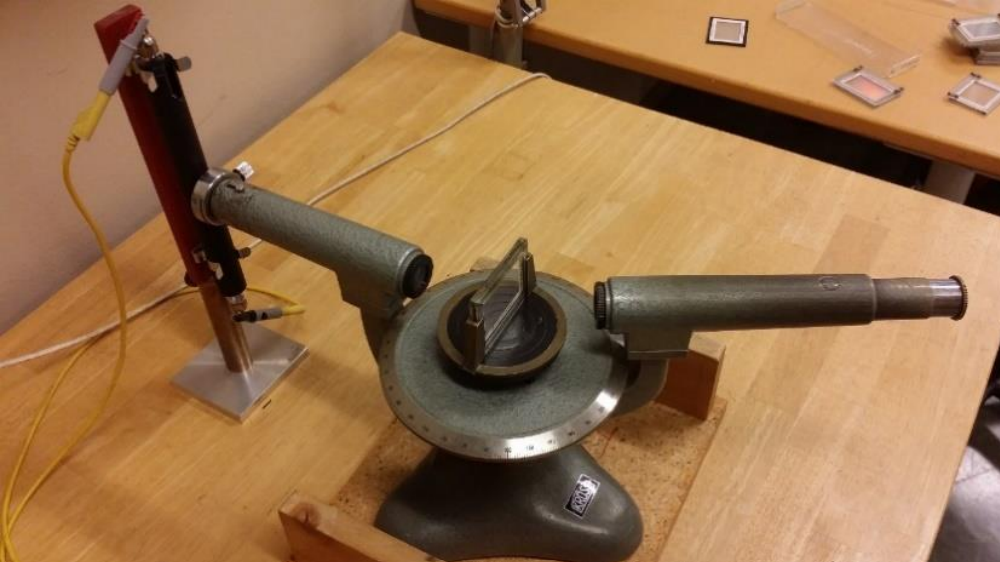
\includegraphics[width = .4\textwidth]{Oppsett_Ba.png}
      \caption{Oppsett for observasjon av spektrallinjer hentet fra \ref{source: lab}}
      \label{fig: Oppsett_Ba}
    \end{figure}
    
    \begin{figure}[h!]
      \centering
      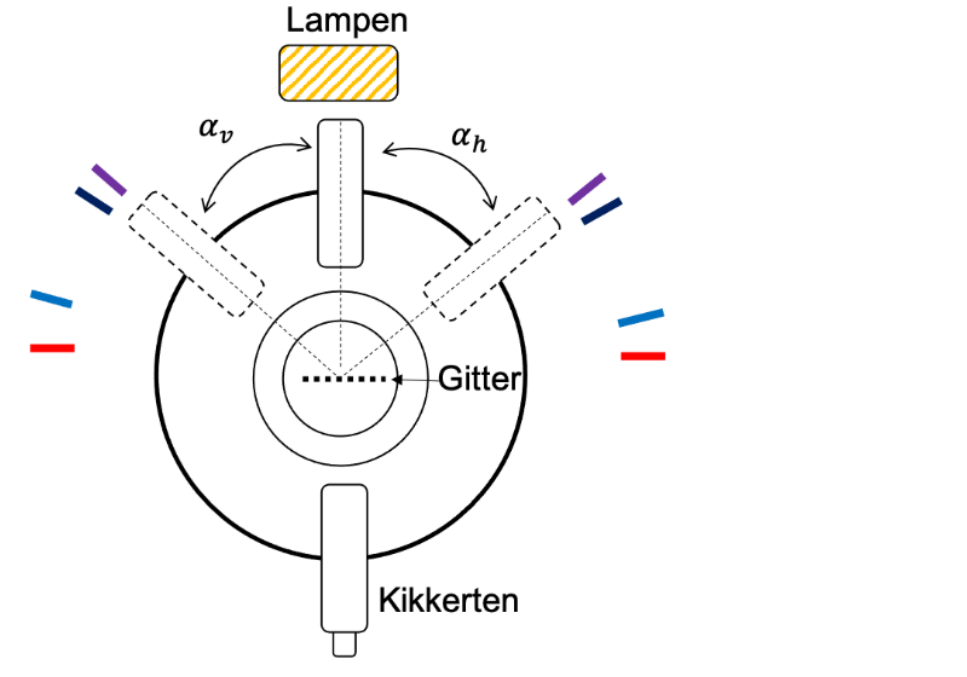
\includegraphics[width = .4\textwidth]{Oppsett_Bb.png}
      \caption{Illustrasjon av oppsett for observasjon av spektrallinjer hentet fra \ref{source: lab}}
      \label{fig: Oppsett_Bb}
    \end{figure}
    Ved å roterer kikkerten som vist i \cref{fig: Oppsett_Bb} finner vi de forskjellige spektrallinjene til Hydrogen. Ved å sikte krysset i kikkerten så sentrert på spektrallinjen som mulig noterer vi oss vinkelen $α$. Dette gjøres på begge sider før vi tar diferansen over to for å få så nøyaktig vinkel som mulig. Vi annslår at vi har en usikkerhet på $1^∘$ ved avlesning.
    Ved bruk av vinkelen kan vi beregne bølgelengden til lyset fra spektrallinjen. Dette sammenlignes med de teoretiske verdiene
    . Vi gjentar prosessen Helium. 
    
    
  \subsection{Zeeman Effekten}
    \begin{figure}[h!]
      \centering
      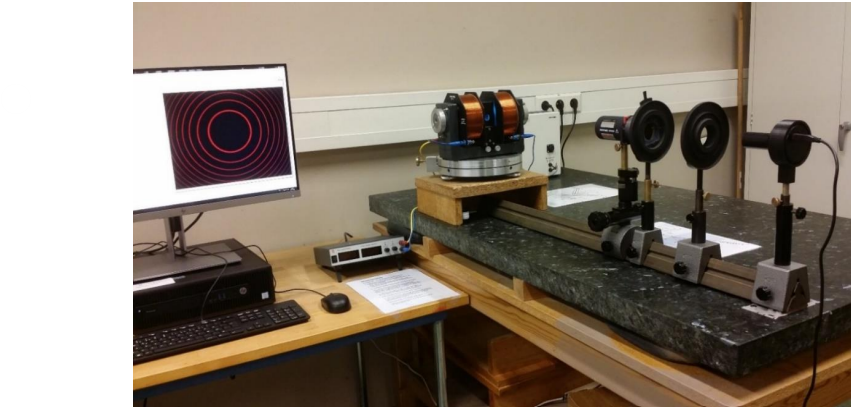
\includegraphics[width = .45\textwidth]{Oppsett_Ca.png}
      \caption{Oppsett for forsøk på Zeeman effekten hentet fra \ref{source: lab}}
      \label{fig: Oppsett_3a}
    \end{figure}
    
    \begin{figure}[h!]
      \centering
      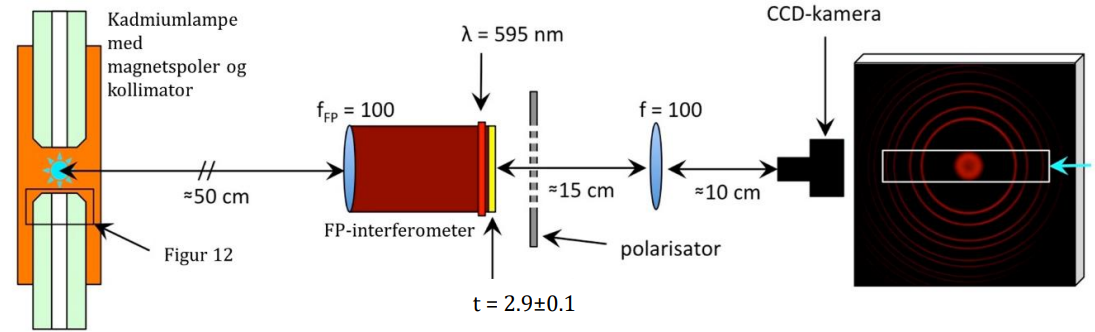
\includegraphics[width = .45\textwidth]{Oppsett_Cb.png}
      \caption{Detaljert illustrasjon for oppsettet ved forsøk på Zeeman effekten hentet fra \ref{source: lab}}
      \label{fig: Oppsett_3b}
    \end{figure}
    % TODO: Legg til kilder og bedre figurtekst
    
    Som vist i figur \cref{fig: Oppsett_3a} og \cref{fig: Oppsett_3b} satt vi opp en Kadmiumlampe i en elektromagnet mellom to spoler. Vi anslår at lyspæren står sentrert $\pm 3$ mm. Spektrallinjene blir oppsplittet i magnetfeltet som resulterer i en interferens vi observerer med et CCD-kamera. 
    % TODO: Utdyp mer av det som står på side 13 og legg til innstillinger i GIMP
    For å sjekke at lyset er planpolarisert ved å rotere polarisasjonsfilteret foran kameraet 90 grader 
    % TODO: Dobbeltsjekk at vinkelen stemmer. 
    og observere at lyset forsvinner. Vi tar et skjermbilde av ringmønsteret for når elektromagneten har en strøm $A = 3$ ampere og $A = 4$ ampere. Deretter bruker vi GIMP til å måle tykkelsen de tre ringene nærmest sentrum. Størrelsene er relative så vi bruker pixler som enhet. Til slutt sammenligner vi vår eksperimentelle verdi av Bohr-magnetonet $μ_B$. 
    
    

\section{Resultater} \label{sec: resultater} 
  \subsection{Diffraksjon og interferens fra forskjellig typer spalter}
  
  I \cref{tabell1} har vi notert ned de målte avstanden $Δx$ fra sentrum av hoved maksima til lys minima. Dette er gjort for de tre første lys minima. Dette resulterer i tre verdier for hver spaltebredde $a ∈ \left\{0.02, 0.04, 0.08, 0.16\right\}$ mm. Vi har også lagt til de utregnede verdiene for $a$ basert på disse avstandene, samt dets usikkerheter. Vi har med intensjon lagt til fler desimaler enn usikkerheten krever ettersom flere av beregningene var såpass nære den teoretiske verdien. 
  
  
  \begin{center}
    %\renewcommand{\arraystretch}{1.2}
    \begin{table}[h]
    \centering
    \begin{tabular}{| C{0.4cm} | C{1.4cm} | C{1.8cm} | C{2.0cm} | C{1.2cm} |}
    \hline
        $n$ & $\Delta x$ [mm] & $a_\text{eksp}$ [mm] & $\Delta a_{\text{eksp}}$ [mm] & $a$ [mm] \\
        \hline
        1 & 15.75 & 0.0231 & 0.0001 & 0.02 \\
        \hline
        2 & 31.00 & $\:\:$0.02352 & $\:\:$0.00009 & 0.02 \\
        \hline
        3 & 47.00 & $\:\:$0.02327 & $\:\:$0.00008 & 0.02 \\
        \hline
        1 & $\:\:$8.00 & 0.0456 & 0.0004 & 0.04 \\
        \hline
        2 & 15.00 & 0.0486 & 0.0003 & 0.04 \\
        \hline
        3 & 23.50 & 0.0465 & 0.0002 & 0.04 \\
        \hline
        1 & $\:\:$4.00 & 0.091$\:\:$ & 0.001$\:\:$ & 0.08 \\
        \hline
        2 & $\:\:$7.50 & 0.0972 & 0.0008 & 0.08 \\
        \hline
        3 & 11.75 & 0.0931 & 0.0006 & 0.08 \\
        \hline
        1 & $\:\:$1.75 & 0.208$\:\:$ & 0.007$\:\:$ & 0.16 \\
        \hline
        2 & $\:\:$3.75 & 0.194$\:\:$ & 0.003$\:\:$ & 0.16 \\
        \hline
        3 & $\:\:$6.00 & 0.182$\:\:$ & 0.002$\:\:$ & 0.16\\
    \hline
    \end{tabular}
    \caption{Her er $\Delta x$ avstanden fra symmetriaksen til $n$-te lysminima, $a_\text{eksp}$ og $\Delta a_\text{eksp}$ er hhv. de eksperimentelt utregnede spaltebreddene og usikkerhetene i disse, mens $a$ er de faktiske spaltebreddene. Alle lengder er oppgitt i mm.}
    \label{tabell1}
    \vspace{-0.7cm}
    \end{table}
    %\renewcommand{\arraystretch}{1}
    \end{center}
    
  
  
    Videre observerte vi at \cref{fig: a4A25,fig: a4A50,fig: a8A25,fig: a8A50} med teoretisk antall lokale maksima stemte overens med hva vi observerte i praksis som sett i \cref{fig: Eksperiment_A2}
       
    \begin{figure}[h!]
      \centering
      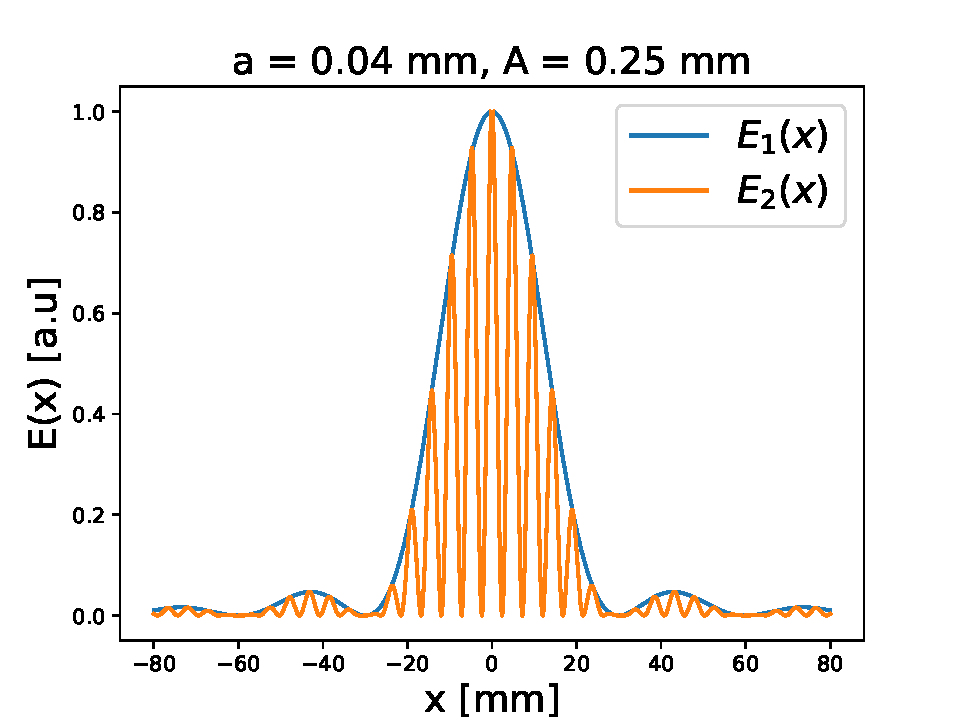
\includegraphics[width = .45\textwidth]{plot_a0.04_A0.25.pdf}
      \caption{Numerisk beregnet plot av relativ teoretisk illuminans. Vi teller 13 lokale lysmaksima innenfor hovedmaksima}
      \label{fig: a4A25}
    \end{figure}
    
    \begin{figure}[h!]
      \centering
      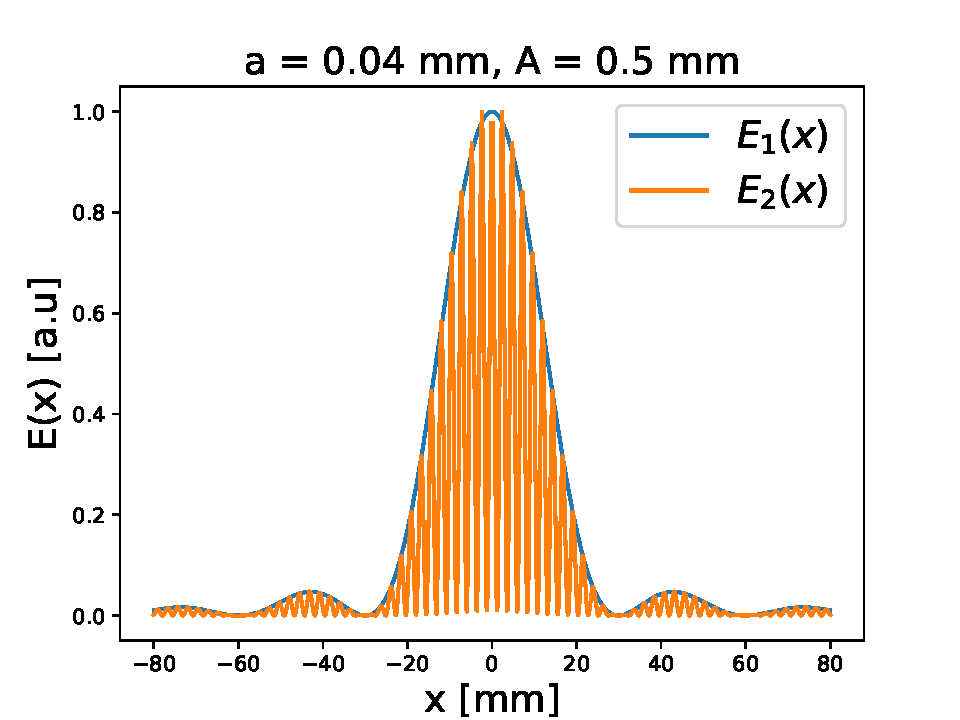
\includegraphics[width = .45\textwidth]{plot_a0.04_A0.5.pdf}
      \caption{Numerisk beregnet plot av relativ teoretisk illuminans. Vi teller 25 lokale lysmaksima innenfor hovedmaksima}
      \label{fig: a4A50}
    \end{figure}
    
    \begin{figure}[h!]
      \centering
      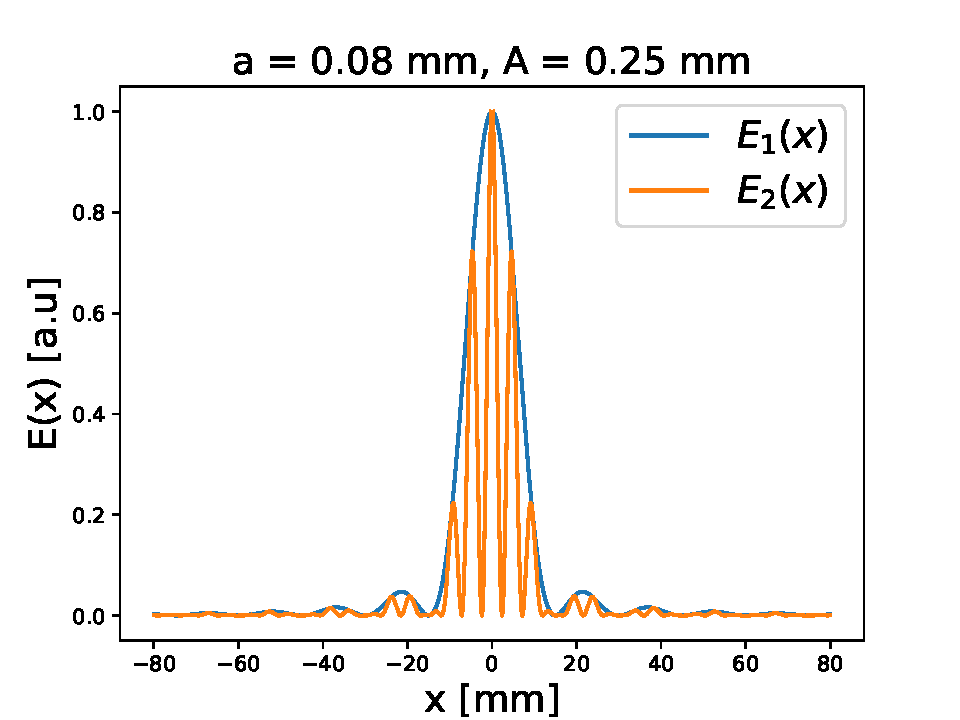
\includegraphics[width = .45\textwidth]{plot_a0.08_A0.25.pdf}
      \caption{Numerisk beregnet plot av relativ teoretisk illuminans. Vi teller 7 lokale lysmaksima innenfor hovedmaksima}
      \label{fig: a8A25}
    \end{figure}
    
    \begin{figure}[h!]
      \centering
      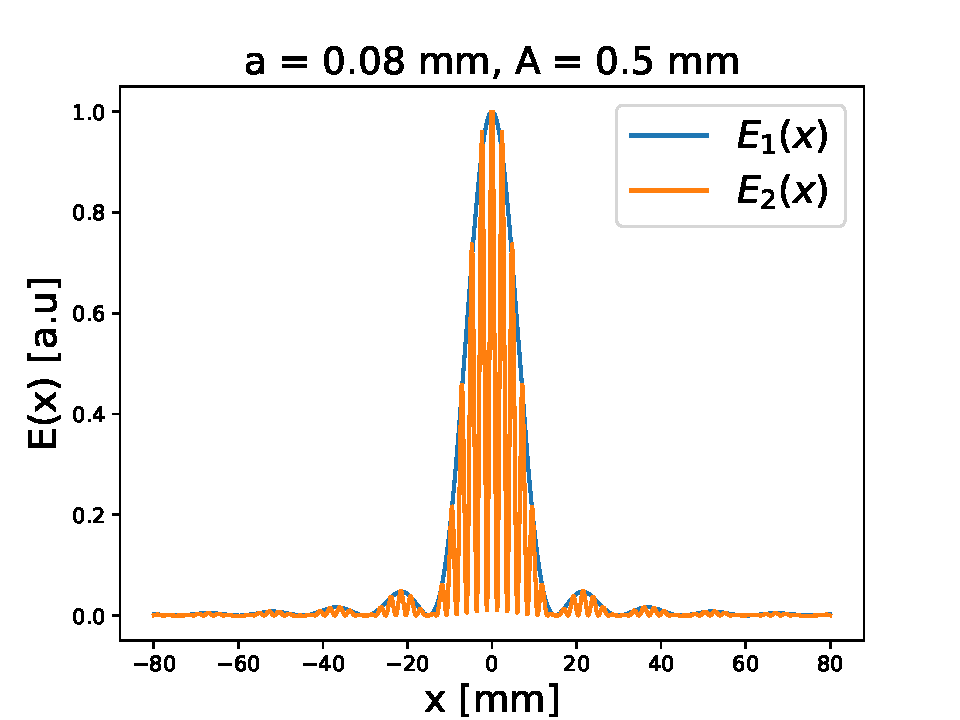
\includegraphics[width = .45\textwidth]{plot_a0.08_A0.5.pdf}
      \caption{Numerisk beregnet plot av relativ teoretisk illuminans. Vi teller 13 lokale lysmaksima innenfor hovedmaksima}
      \label{fig: a8A50}
    \end{figure}
    
    \begin{figure}[h!]
      \centering
      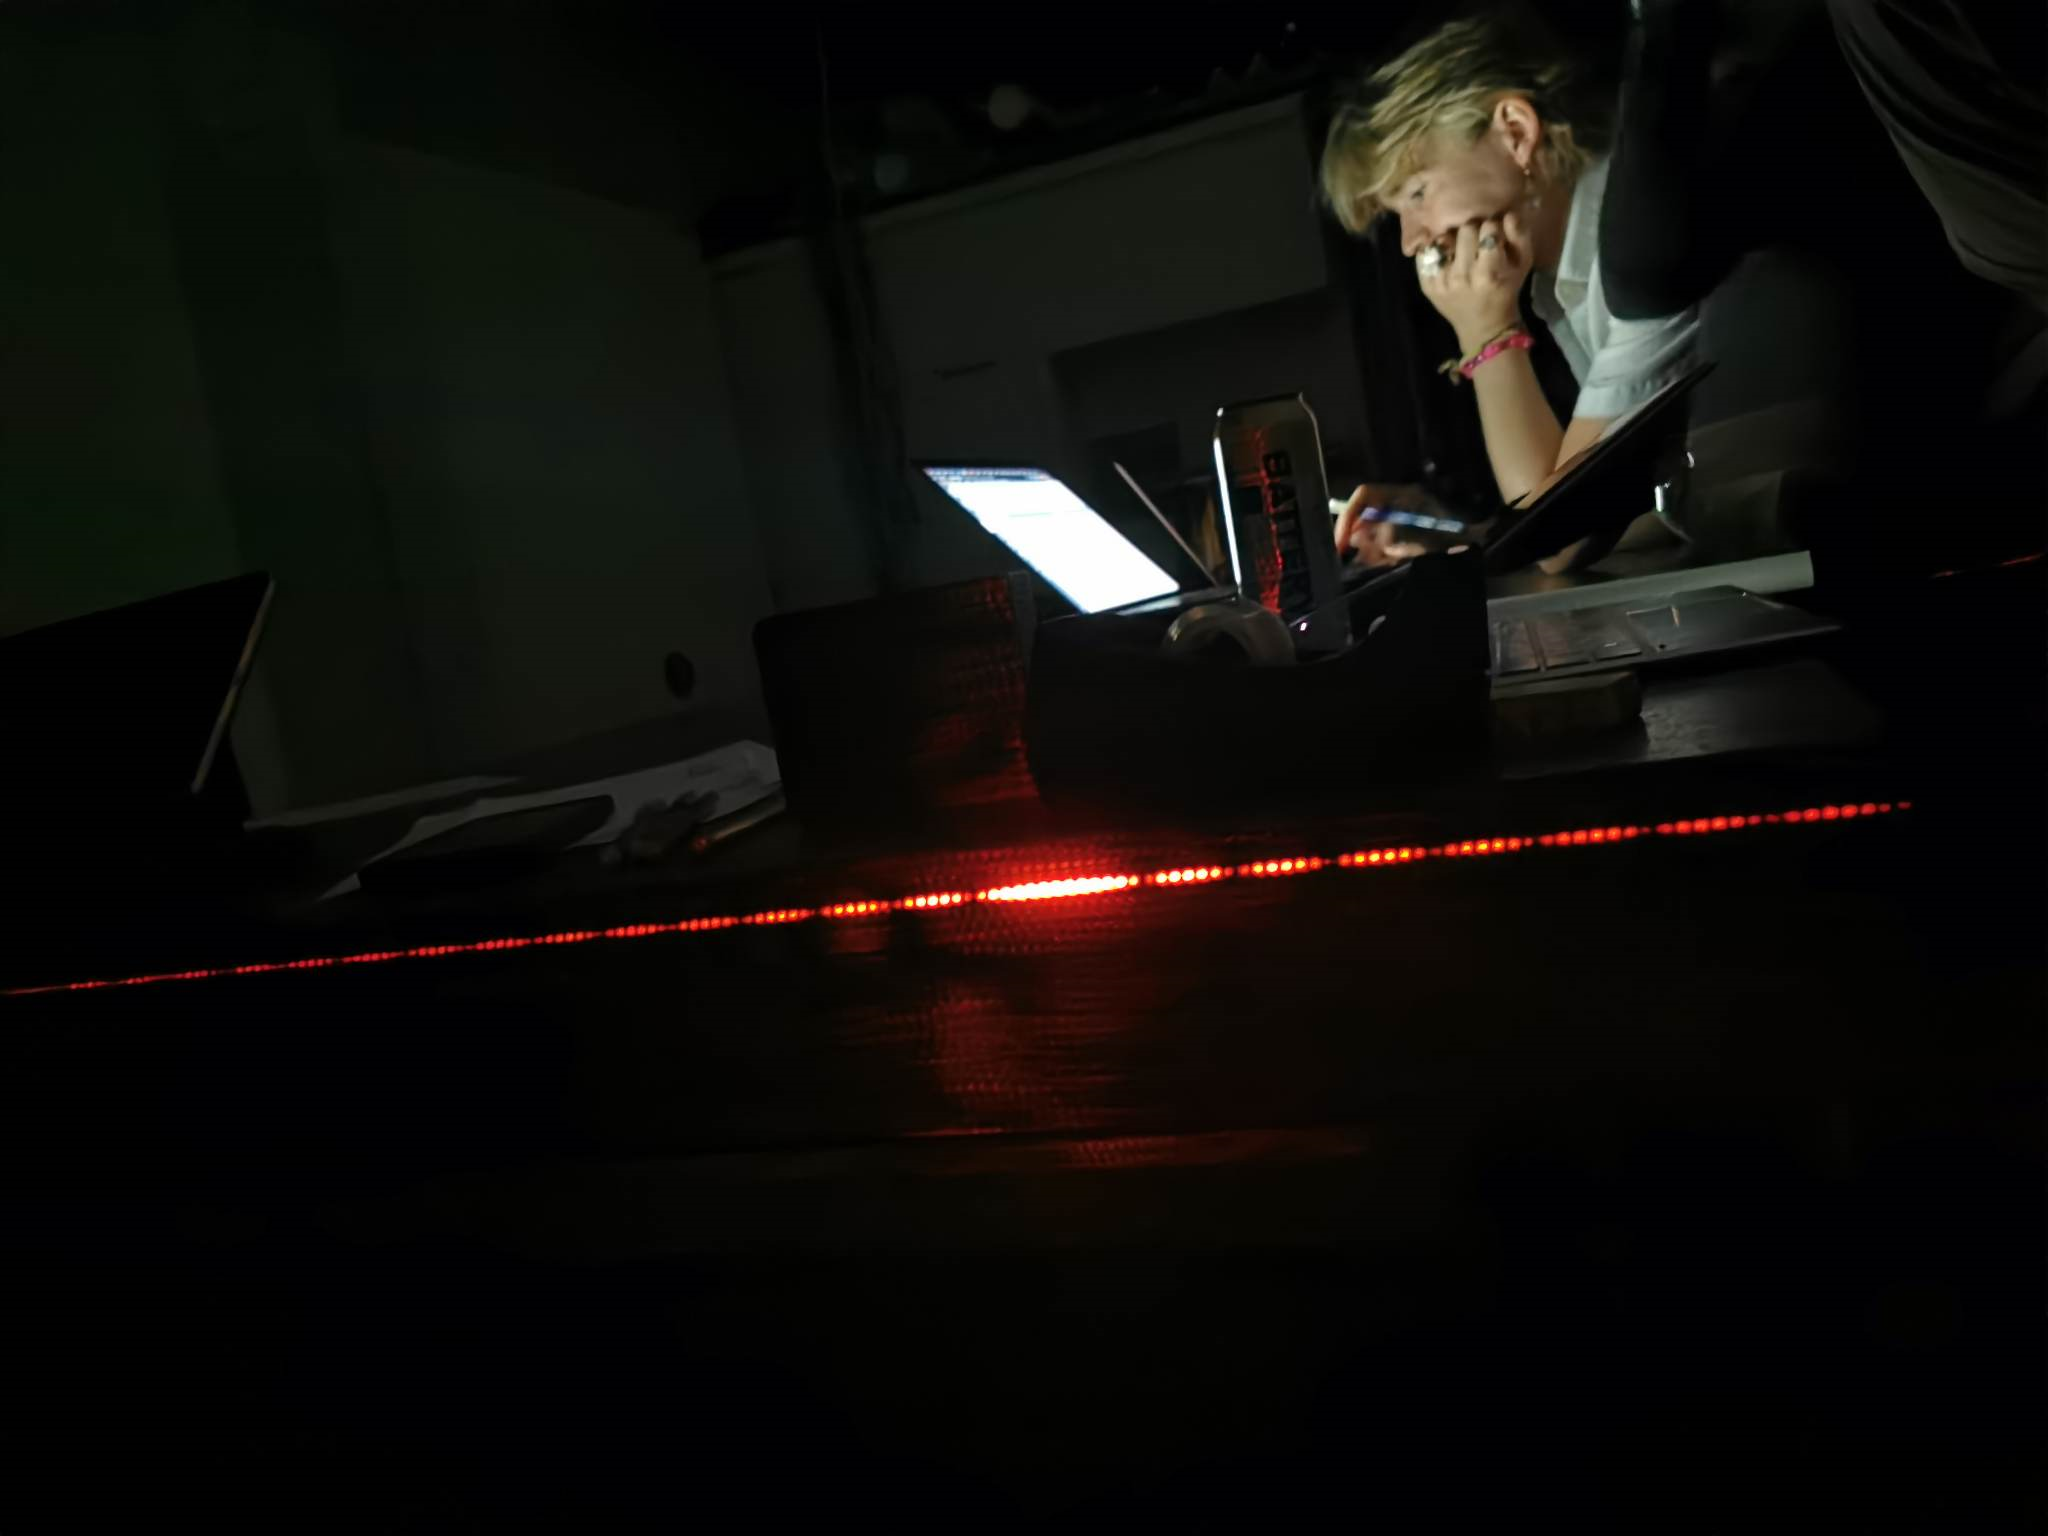
\includegraphics[width = .45\textwidth]{Eksperiment_A2.png}
      \caption{Eksperimentelle interferensmønster. Vi kunne enkelt telle 13 lokale lysmaksima ved $a=0.08$ mm og $A = 0.5$ mm}
      \label{fig: Eksperiment_A2}
    \end{figure}
    
    
    Vi har noter i \cref{tabell2} den målte diameteren $d_{\text{mål}}$ til den $n$-te mørke ringen, for de forskjellige sirkulære aperturene. I samme tabell har vi lagt til teoretisk beregnet aperturdiameter og dets usikkerhet. 
    
    \begin{center}
  \begin{table}[h]
    \centering
    \begin{tabular}{| C{2.0cm} | C{0.5cm} | C{1.5cm} | C{1.8cm} | C{1.9cm} |}
      \hline
      $d_\text{apertur}$ [mm] & $n$ & $d_\text{mål}$ [mm] & $d_\text{teori}$ [mm] & $\Delta d_\text{teori}$ [mm] \\
      \hline
      0.2 & 1 & 13.0 & 14.62 & 0.02 \\
      \hline
      0.2 & 2 & 24.9 & 26.77 & 0.03 \\
      \hline
      0.2 & 3 & 36.0 & 38.81 & 0.04 \\
      \hline
      0.4 & 1 & $\:\:$6.6 & $\:\:$7.31 & 0.01 \\
      \hline
      0.4 & 2 & 12.6 & 13.38 & 0.01 \\
      \hline
      0.4 & 3 & 18.5 & 19.41 & 0.02 \\
  \hline
  \end{tabular}
  \caption{Målt diameter $d_\text{mål}$ til den $n$-te mørke ringen i diffraksjonsmønstrene er oppgitt i mm, både for det sirkulære aperturet med diameter $d_\text{apertur} = 0.2\:$mm og med diameter $d_\text{apertur} = 0.4\:$mm. De teoretiske diameterne som er regnet ut ifra avstanden $R$ mellom apertur og skjerm er oppgitt sammen med usikkerheten i disse, begge i mm.}
  \label{tabell2}
  \vspace{-0.7cm}
  \end{table}
  \end{center}  
  
  
  \subsection{Gitterspektrometri}
    
  I \cref{tabell3} er det notert de målte vinklene $α_h$ og $α_v$ samt gjennomsnittlig vinkel avstand fra sentralaksen $θ$ fra vi observerte Hydrogenet. Vi har også regnet ut bølgelengden til lyset og sammenlignet med teoretiske verdier. Hydrogenet har spektrallinje for $λ = 397.042$ nm, som vi naturligvis ikke kunne observere med det blotte øye. Det samme er gjort for Helium i \cref{tabell4}. Én av de teoretiske bølgelengdene klarte vi ikke å observere for $λ = 402.6$ nm, ettersom den var for mørk. 
  \begin{center}
    \begin{table}[h]
    \centering
    \begin{tabular}{| C{1.1cm} | C{1.1cm} | C{1.1cm} | C{1.1cm} | C{1.3cm} | C{1.7cm} |}
    \hline
        $\alpha_h$ & $\alpha_v$ & $\theta$ & $\lambda$ [nm] & $\Delta \lambda$ [nm] & $\lambda_\text{teori}$ [nm] \\
        \hline
        244.0$^\circ$ & 142.5$^\circ$ & 50.8$^\circ$ & 656 & 3 & 656.335 \\
        \hline
        228.5$^\circ$ & 158.5$^\circ$ & 35.0$^\circ$ & 486 & 4 & 486.174 \\
        \hline
        224.0$^\circ$ & 162.5$^\circ$ & 30.8$^\circ$ & 433 & 5 & 434.084 \\
        \hline
        222.0$^\circ$ & 164.5$^\circ$ & 28.8$^\circ$ & 407 & 5 & 410.210 \\
    \hline
    \end{tabular}
    \caption{Avleste vinkler $\alpha_h$ og $\alpha_v$, samt de beregnede vinklene $\theta$ som vi fant fra disse, alle tre i grader. Bølgelengdene vi regnet ut og usikkerheten i disse, samt de teoretisk utregnede bølgelengdene $\lambda_\text{teori}$ for emisjonsspekteret til hydrogen er oppgitt i nanometer.}
    \label{tabell3}
    \vspace{-0.7cm}
    \end{table}
    \end{center}
    
    \begin{center}
      \begin{table}[h]
      \centering
      \begin{tabular}{| C{1.1cm} | C{1.1cm} | C{1.1cm} | C{1.1cm} | C{1.3cm} | C{1.7cm} |}
      \hline
          $\alpha_h$ & $\alpha_v$ & $\theta$ & $\lambda$ [nm] & $\Delta \lambda$ [nm] & $\lambda_\text{teori}$ [nm] \\
          \hline
          255.0$^\circ$ & 151.0$^\circ$ & 52.0$^\circ$ & 667 & 3 & 667.8 \\
          \hline
          249.0$^\circ$ & 161.0$^\circ$ & 44.0$^\circ$ & 588 & 4 & 587.5 \\
          \hline
          240.5$^\circ$ & 168.0$^\circ$ & 36.3$^\circ$ & 501 & 4 & 501.5 \\
          \hline
          239.5$^\circ$ & 168.5$^\circ$ & 35.5$^\circ$ & 492 & 4 & 492.1 \\
          \hline
          238.0$^\circ$ & 170.0$^\circ$ & 34.0$^\circ$ & 474 & 4 & 471.3 \\
          \hline
          236.0$^\circ$ & 172.0$^\circ$ & 32.0$^\circ$ & 449 & 4 & 447.1 \\
      \hline
      \end{tabular}
      \caption{Avleste vinkler $\alpha_h$ og $\alpha_v$, sammen med vinklene $\theta$ som vi fant fra disse. Alle vinklene er oppgitt i grader. Bølgelengdene vi regnet ut og usikkerheten i disse, samt de teoretisk utregnede bølgelengdene $\lambda_\text{teori}$ for emisjonsspekteret til helium er oppgitt i nanometer.}
      \label{tabell4}
      \vspace{-0.7cm}
      \end{table}
      \end{center}
      
    
    % Vi beregnet også gitteret sin oppløsningsevne gitt ved , til å være 
    % \[
    % \frac{λ}{Δλ} = 1 ⋅ (30\ 000 ± 1) = 30\ 000 ± 1
    % \]
    
  
  \subsection{Zeeman-effekten}
  
  Notert i \cref{tabell5} er de målte indre og ytre diameteren hentet ut fra måleprogrammet GIMP, strømmen $I$ brukt, og gjennomsnittsdiameteren $d_i$. Ved $I = 3$ A, observerte vi diffraksjonsmønsteret sett i \cref{fig: 3I}. Ved $I = 4$ A Observerte vi diffraksjonsmønsteret sett i \cref{fig: 4I}.
      
  \begin{center}
    \begin{table}[H]
    \centering
    \begin{tabular}{| C{0.8cm} | C{0.5cm} | C{1.2cm} | C{1.2cm} | C{1.2cm} |}
    \hline
        $I$ [A] & $i$ & $d_i^-$ & $d_i^+$ & $d_i$ \\
        \hline
        3 & 1 & 380 & 402 & 391.0 \\
        \hline
        3 & 2 & 456 & 475 & 465.5 \\
        \hline
        3 & 3 & 605 & 620 & 612.5 \\
        \hline
        4 & 1 & 367 & 392 & 379.5 \\
        \hline
        4 & 2 & 463 & 485 & 474.0 \\
        \hline
        4 & 3 & 598 & 614 & 606.0 \\
    \hline
    \end{tabular}
    \caption{Indre ($d_i^-$) og ytre ($d_i^+$) diameter for $i$-te lysmaksima unna sentrum av sirklene både når strømmen var på $I = 3\:$A og når den var på $I = 4\:$A, samt estimatet $d_i$ vi fikk fra disse. Diameterne er målt i piksler med måleverktøyet GIMP.}
    \label{tabell5}
    \vspace{-0.7cm}
    \end{table}
    \end{center}
    
  \begin{figure}[h!]
    \centering
    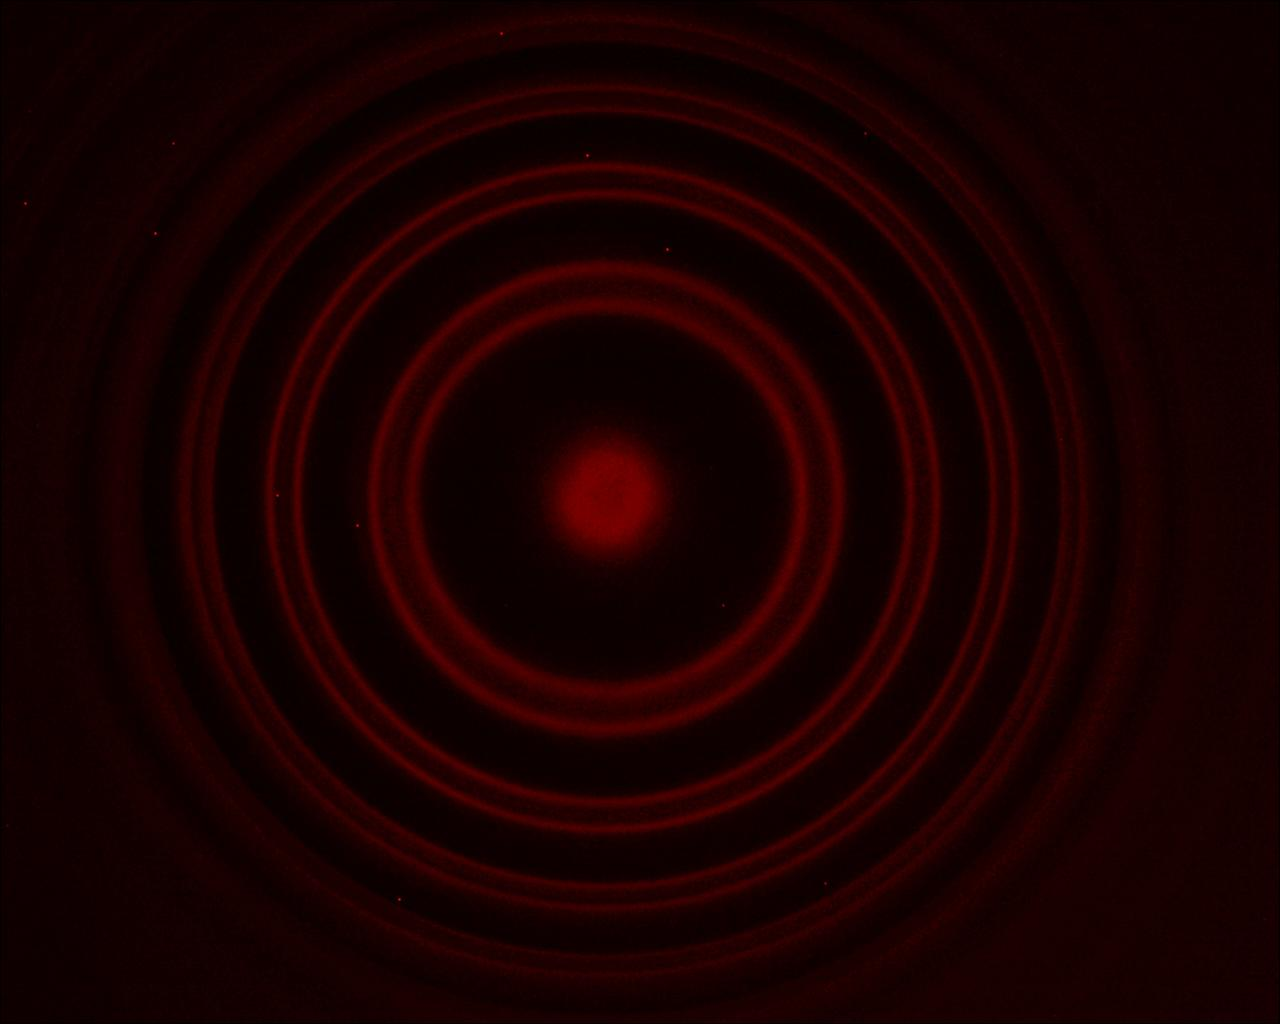
\includegraphics[width = .45\textwidth]{3amp.jpg}
    \caption{Diffraksjonsmønster ved $I = 3$ A.}
    \label{fig: 3I}
  \end{figure}
  
  \begin{figure}[h!]
    \centering
    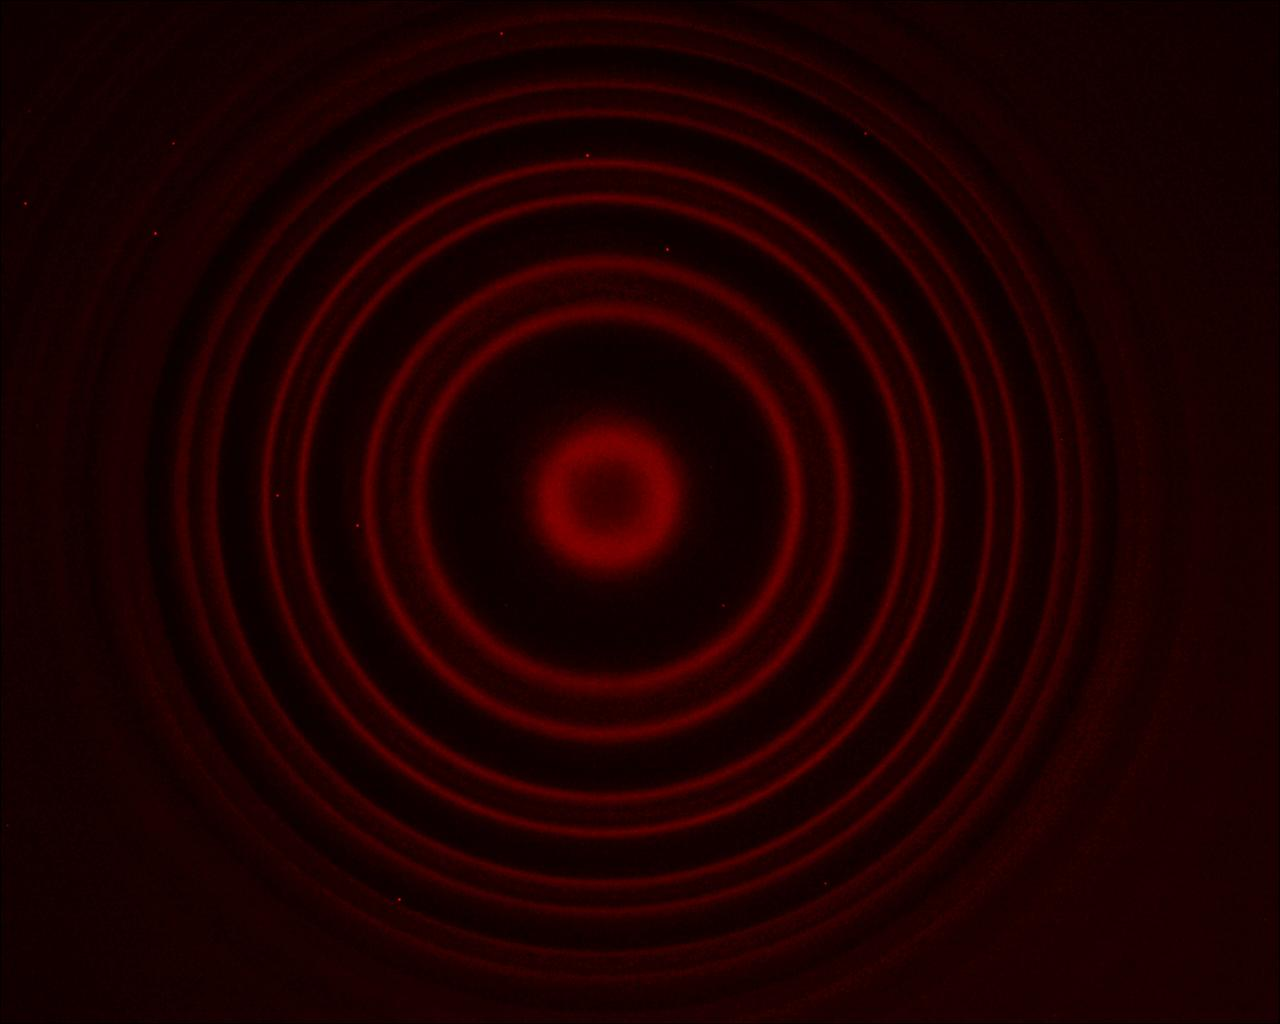
\includegraphics[width = .45\textwidth]{4amp.jpg}
    \caption{Diffraksjonsmønster ved $I = 4$ A.}
    \label{fig: 4I}
  \end{figure}
  
  \subsubsection*{3 Ampere strøm}
    Ved å sette \cref{eq: nokkelparameter 3} inn i \cref{eq: delta nu} beregner vi frekvensforsjkellen $Δν$ til å være \cref{eq: delta nu 3}, som gir et Bohr-magneton på \cref{eq: Bohr magneton 3}.
    
    \begin{equation}\label{eq: nokkelparameter 3}
      δ = 0.29 ± 0.02
    \end{equation}

    \begin{equation}\label{eq: delta nu 3}
      Δν = (1.9 ± 0.1) ⋅ 10^{10} \text{ Hz}
    \end{equation}
    
    \begin{equation}\label{eq: Bohr magneton 3}
      μ_B = (8.9 ± 0.5) ⋅ 10^{-24} \text{ J/T}
    \end{equation}
  
  \subsubsection*{4 Ampere strøm}
    Vi gjentar stegene for $I = 4$ A, og får \cref{eq: nokkelparameter 4,eq: delta nu 4,eq: Bohr magneton 4}.
      
    \begin{equation}\label{eq: nokkelparameter 4}
      δ = 0.36 ± 0.02      
    \end{equation}
    
    \begin{equation}\label{eq: delta nu 4}
      Δν = (1.9 ± 0.1) ⋅ 10^{10} \text{ Hz}      
    \end{equation}
    
    \begin{equation}\label{eq: Bohr magneton 4}
      μ_B = (8.9 ± 0.5) ⋅ 10^{-24} \text{ J/T}
    \end{equation}
  
    


\section{Diskusjon} \label{sec: diskusjon}
  \subsection{Diffraksjon og interferens fra forskjellig typer spalter}
  % TODO: I A.1, nevn hvordan beregnet a, blir mer og mer feil, når d øker ettersom avstanden mellom lysminima minker og dermed blir den relative usikkerheten større. 
  
  For de beregnede verdiene fikk vi såpass presise resultater at vi så det nødvendig å inkludere flere gjeldene siffer enn det vi egentlig kunne, ettersom vi ønsket å vise at våre beregninger ikke sammenfallt fullstendig med de teoretiske verdiene. Et interessant funn, er hvordan vi får en økning i vår feil, når spaltestørrelsen $a$ øker. Det gir mening ettersom vi har en konstant tilfeldig usikkerhet i målingene av distanse ved bruk av skyvelæra. Når $a$ øker, vil avstanden mellom lysminima minker, og dermed blir den relative usikkerheten større. Denne trenden ser en klart i \cref{tabell1} sin kolonne for $Δa$, hvor usikkerheten øker betraktelig for hver teoretiske verdi $a$. I tilegg til kortere distanse å måle, kan det også ha vært litt vanskeligere å se lysminimaene hvis de mørke områdene blir veldig små. Ved å beregne standardavviket til gjennomsnittsmålingene ser vi igjen tydelig at usikkerheten øker med økende $a$, som notert i \cref{tabell6}
  
  \begin{center}
    \begin{table}[h]
    \centering
    \begin{tabular}{| C{2.0cm} | C{2.4cm} | C{1.6cm} |}
    \hline
        $\overline{a}_\text{exp}$ [mm] & SE($\overline{a}_\text{exp}$) [mm] & $a$ [mm] \\
        \hline
        0.0233 & 0.0001 & 0.02 \\
        \hline
        0.0469 & 0.0009 & 0.04 \\
        \hline
        0.094$\:\:$ & 0.002$\:\:$ & 0.08 \\
        \hline
        0.195$\:\:$ & 0.008$\:\:$ & 0.16 \\
    \hline
    \end{tabular}
    \caption{Gjennomsnittene $\overline{a}_\text{exp}$ av de eksperimentelt beregnede spaltebreddene, standardavvikene SE($\overline{a}_\text{exp}$) av disse gjennomsnittene, og de faktiske spaltebreddene $a$. Alle verdiene er i mm.}
    \label{tabell6}
    \vspace{-0.7cm}
    \end{table}
    \end{center}
    
    
  Ved bruk av dobbeltspalter sammenfalt teoretiske og eksperimentelle verdier akkurat som de skulle. Vi kunne i alle tilfeller enkelt telle forutsett lokale lysminima. Dette kunne en til og med telle fra et bilde av interfernsmønsteret som sett i \cref{fig: Eksperiment_A2}

  Vi oppdaget at de målte diameterene til de mørke ringene var ca. 1 mm mindre enn de teoretiske verdiene. Likevel estimerte vi selv en usikkerhet på $0.1$ mm for de målte verdiene. Vi undersøkte dette dypere ved å se om usikkerhetene muligens kunne "overlappe" slik at denne feilen kunne forklares. Dette er notert i \cref{tabell7}. Likevel ser vi at dette ikke stemmer og usikkerhetene kan ikke forklares av dette alene. Vi har mest sannsynlig undervurdert vår egen feil i selve målingen, ettersom både upresis plassering av skyvelæret samt upresis markering ved tusj kan ha hatta større effekt enn antatt. Likevel ser vi samme fenomen som ved enkeltspalte, at vi har mindre feil, ved større aperturdiameter. Dette kan forklares med at interferensmønsteret produserer ringer med bredere lysmaksima, som gjør det lettere å måte fra sentrum til de mørke områdene. Lenger unna sentrum ble det observert at ringene ble mer utydelige, og det var vanskeligere å måle diameteren. Dette kan også ha bidratt til feilen.
  
  
  \begin{center}
    \begin{table}[H]
    \centering
    \begin{tabular}{| C{2.0cm} | C{2.0cm} | C{2.8cm} |}
    \hline
        $d_\text{mål}^+$ [mm] & $d_\text{teori}^-$ [mm] & $d_\text{teori}^- - d_\text{mål}^+$ [mm] \\
        \hline
        13.1 & 14.60 & 1.5 \\
        \hline
        25.0 & 26.74 & 1.7 \\
        \hline
        36.1 & 38.77 & 2.7 \\
        \hline
        $\:\:$6.7 & $\:\:$7.30 & 0.6 \\
        \hline
        12.7 & 13.37 & 0.7 \\
        \hline
        18.6 & 19.39 & 0.8 \\
    \hline
    \end{tabular}
    \caption{Her er $d_\text{mål}^+ = d_\text{mål} + \Delta d_\text{mål}$ den største mulige verdien av de målte diameterne med usikkerheten vi estimerte, og $d_\text{teori}^- = d_\text{teori} - \Delta d_\text{teori}$ minste mulige verdi av de teoretisk beregnede diameterne med tanke på de beregnede usikkerhetene til hver av dem. Siden $d_\text{mål}$ er oppgitt med nøyaktighet på kun ett desimal, har jeg oppgitt differansen mellom de to med samme nøyaktighet. Alle størrelsene er i mm.}
    \label{tabell7}
    \vspace{-0.7cm}
    \end{table}
    \end{center}


  \subsection{Gitterspektroskopi}
    Selv om flere av linjene var vanskelig å få øye på, var det enkelt å plassere trådkorset på dem når de først var funnet. En kunne ha satt usikkerheten i notasjonen til vinkelen $α_h$ eller $α_v$ til å $1^∘$, men vi valgte å holde det en konstant $0.5^∘$ for alle. Dette fungerte helt fint ettersom vi i de fleste tilfellene bare bommet med $<1$ nm. Kortere bølgelengder hadde større avvik fra teoretisk verdi, men de hadde også mindre avbøyningsvinkel som gjør vår evne til å plassere trådkorset samt lese av vinkelen en større kilde til feil. En mulig feilkilde kunne ha vært opppløsningsevnen til gitteret, men ved bruk av \cref{eq: gitter opplosning} på største å minste bølgelengde, finner vi den mulig feilen fra dette som sett i \cref{eq: gitter opplosning max,eq: gitter opplosning min} at er neglisjerbart.
    
    \begin{equation}\label{eq: gitter opplosning max}
      Δλ_{\text{max}} ≈ 0.022 \text{ nm}
    \end{equation}
    
    \begin{equation}\label{eq: gitter opplosning min}
      Δλ_{\text{min}} ≈ 0.014 \text{ nm}
    \end{equation}



  \subsection{Zeeman-effekten}
    Utstyret brukt i eksperimentet var ekstremt sensitivt. Vi kunne derfor ikke måle nøyaktig plassering av kadmiumlampen mellom elektromagnetene. Det gjør at usikkerheten i magnetfeltstyrken er vanskeligere å bestemme. På øyemål anslo vi at usikkerheten måtte være på ca. 3 mm. Som sett i 
    % TODO: referer til kallibreringskurven
    var det stor forskjell på $B^{+}$ og $B^{-}$ at vi heller ville være på den sikre siden. Likevel kunne vi se større frekvensforskjell $Δν$ med strømmen $I = 4$ A enn for $I = 3$ A, som forventet. Økt strøm gir økt magnetfeltstyrke som skal føre til tydeligere Zeeman-effekt. Den beregnede verdien for Bohr-magneton var feil med bare $0.55\%$ ved $I = 3$ A, og $3.86\%$ for $I = 4$. Dette er litt overraskende ettersom en skulle tenkt at lavere strøm gjorde at avstandene mellom ringene ble mindre, som ville gjort at vår evne til å bruke GIMP nøyaktig ville skapt større relativ usikkerhet. Likevel ser vi at om vi sammenligner vårt avvik fra den teoretiske verdien \cref{eq: bohr avvik}, er den innenfor usikkerhetene vår \cref{eq: bohr usikkerhet}
    
    \begin{equation}\label{eq: bohr avvik}
      \Delta \mu_B = \left|\mu_{B,\text{eksp}} - \mu_{B,\text{tabell}}\right| \approx 0.4\times 10^{-24}\:\text{J/T}  
    \end{equation}
    
    \begin{equation}\label{eq: bohr usikkerhet}
      \Delta \mu_{B,\text{eksp}} \approx 0.5 \times 10^{-24}\:\text{J/T}    
    \end{equation}
  



\section{Konklusjon} \label{sec: konklusjon}
Etter å ha observert de kvantemekaniske egenskapene til lys som både bølge og partikkel fra diffraksjon og emisjon har vi vært vellykket i å teste de teoretiske konseptene rundt dette. Vi har observert hvordan diffraksjonsmønster endres ved forskjellige typer spalter og hvordan dimensjonene til til disse spaltene påvirker mønsteret. Det var tydelig at ved mindre $a$, fikk vi økt avstand mellom lysminima, og at ved økt $A$ fikk vi flere lokale lysmaksima innenfor hovedmaksima. Vi observerte forventet antall lokale lysmaksima innenfor hovedmaksima som forutsett fra illuminansfunksjonen. Ringene skapt av laser som passerte sirkulært apertur var ikke like enkelt å måle til å være som forventet av teoretiske verdier. Vi undervurderte nok vår egen feil i målingene. Likevel var det klart at større aperturdiameter førte til tynnere mørke ringer som var enklere å måle. 

Balmerlinjene og heliumlinjene ble kalkulert til å være veldig nære de teoretiske verdiene. Noen av linjene var utenfor det synlige spektrumet eller for svake til å se. Her måtte vi ha tatt i bruk mer avansert utstyr for å kunne observere disse. Ellers var avviket mindre enn usikkerhetene så dette var vellykket. 


Ved observasjon av den normale Zeeman-effekten klarte vi å beregne oss tilbake til Bohr-magneton innenfor usikkerhetene våre i forsøket. Vi så klart effekten av magnetfeltet på oppsplittelsen av de degenererte energinivåene ettersom avstanden mellom linjene økte ved høyere strøm. Akkurat som forventet. 


% TODO: Sjekk at rendrer
\section*{References} \label{sec: references}
\begin{enumerate}[label=\Roman*.]
  \item\label{source: lab} Fysisk Institutt, UiO, Revidert Lütken, C. og Read, A. vår 2019, Edin, N. og Markova, M. vår 2022, Oppgaveteksten: Labøvelse FYS2150 Bølgeoptikk.
  \item\label{source: squire} Squires Gordon L. Practical Physics - 4th Edition. Cambridge University Press, 2001.
  \item\label{source: diffraction} \href{https://cdn.instrumentationtools.com/wp-content/uploads/2018/02/diffraction-grating.png}{Instrumental Tools}
  \end{enumerate}

\end{document}